\documentclass[12pt,twocolumn]{article}
\usepackage{amsmath,amsfonts,amssymb}
\usepackage{bm}
\usepackage{empheq}
\usepackage{setspace}
\usepackage{float}
\usepackage{tocloft}
\usepackage{cuted}
\usepackage{flushend}
\usepackage[scaled]{beramono}
\usepackage[T1]{fontenc}
\usepackage{cite}
\usepackage{amsthm}
\usepackage{authblk}
\usepackage[toc,page]{appendix} % for appendices
\usepackage{gensymb}            % for degree symbol
\usepackage[pdftex]{graphicx}   % for figures
\usepackage{siunitx}            % for si units
\usepackage[caption=false]{subfig}  % for subfigures
\usepackage{algorithm}
\usepackage{algpseudocode}
\usepackage{titling}
\usepackage{hyperref}
\usepackage{epstopdf}
\usepackage{esint}
\usepackage{physics}
\hypersetup{
    colorlinks=true,
    urlcolor=blue,
    linkcolor=blue,
    citecolor=red}
\providecommand{\keywords}[1]{\textbf{\textbf{Keywords:~}} #1}
\captionsetup[subfigure]{labelformat=brace} % setup subfigure captions
\graphicspath{{./Figures/}}     % figures in the Figures directory
\DeclareGraphicsExtensions{.eps,.ps,.pdf}    % extensions for figures
\newtheorem{theorem}{Theorem}
\newtheorem{lemma}{Lemma}
\newcommand{\comment}[1]{}      % command for multiline comments
\setlength\stripsep{3pt plus 1pt minus 1pt}
\renewcommand{\cftdotsep}{\cftnodots}
\cftpagenumbersoff{figure}
\cftpagenumbersoff{table}
\begin{document}
\title{A Finite Difference Time Domain Method for Two Dimensional Electromagnetic Wave Propagation In Heterogeneous Lossy Dielectric Media With a Perfectly Matched Layer Boundary Condition}
\author{Patrick D. Cook}
\affil{Department~of~Physics,~Fort~Hays~State~University,\\Hays,~Kansas~67601,~USA}
\date{Fall 2019}
\begin{titlingpage}
\maketitle
\begin{abstract}
In this work, the foundations behind the one- and two-dimensional finite-difference time-domain (FDTD) method in the context of electromagnetic wave propagation are presented. Heterogeneous propagation media with arbitrary dielectric constants and arbitrary electrical conductivities are considered. Different boundary conditions, hard boundaries, cyclic boundaries, and the perfectly matched layer (PML), are presented and discussed. This work includes implementations of the method using both cyclic and PML boundary conditions, written in standard Python 3. These implementations are used to explore a variety of simple and complex geometries.
\end{abstract}

\keywords{Electromagnetic wave simulation, finite-difference time-domain, perfectly matched layer}
\end{titlingpage}
\newpage
\section{Introduction}
The goal of the finite-difference time-domain (FDTD) method is to simulate the propagation of electromagnetic waves in complex geometry. For instance, propagation through several different materials with different dielectric constants, or electrical conductivities. Problems such as these are often impossible to solve analytically, and so numerical approaches, such as this one, are required.

This work is an overview of the derivation of the necessary expressions used in the FDTD method as well as two types of boundary conditions. Implementations of the method for both boundary conditions with results are presented and discussed.
\section{Governing Equations for Electromagnetic Waves}
The differiential form of Maxwell's equations for the electric field, $\mathbf{E}$, and magnetic field, $\mathbf{B}$, in vacuum, are~\cite{Jackson99}
\begin{subequations}
\begin{align}
\div{\mathbf{E}} &= \frac{\rho}{\varepsilon_0}, \\
\div{\mathbf{B}} &= 0, \\
\label{eq:curl_E}\curl{\mathbf{E}}&= -\frac{\partial\mathbf{B}}{\partial t}, \\
\label{eq:curl_B}\curl{\mathbf{B}}&= \mu_0\mathbf{J}+\frac{1}{c^2}\frac{\partial\mathbf{E}}{\partial t}.
\end{align}
\end{subequations}
Where
\begin{itemize}
\item $\rho$ is the free electric charge density
\item $\mathbf{J}$ is the free current density
\item $\varepsilon_0$ is the permittivity of free space
\item $\mu_0$ is the permeability of free space
\item $c$ is the speed of light, $c\equiv\frac{1}{\sqrt{\varepsilon_0\mu_0}}$
\end{itemize}
In the context of electromagnetic wave propagation, only Eqs.~\ref{eq:curl_E}~and~\ref{eq:curl_B} are of interest. Assuming there is no free current, rewriting these two equations in terms of the magnetic field strength, $\mathbf{H}=\mathbf{B}/\mu_0$, and subsituting $c\equiv\frac{1}{\sqrt{\varepsilon_0\mu_0}}$ yields
\begin{subequations}
\begin{align}
\label{eq:dH_dt_vacuum}\frac{\partial\mathbf{H}}{\partial t} &= -\frac{1}{\mu_0}\curl{\mathbf{E}}, \\
\label{eq:dE_dt_vacuum}\varepsilon_0\frac{\partial\mathbf{E}}{\partial t} &= \curl{\mathbf{H}}.
\end{align}
\end{subequations}
In a dielectric medium, we introduce the relative permittivity, $\varepsilon_r$, which is material-specific. This allows us to write the permittivity as $\varepsilon=\varepsilon_r\varepsilon_0$. We could also introduce the relative permeability, but in this work we will assume all materials are nonmagnetic, meaning $\mu_r=1$ and so $\mu=\mu_0$. Eqs.~\ref{eq:dH_dt_vacuum}~and~\ref{eq:dE_dt_vacuum} become
\begin{subequations}
\begin{align}
\frac{\partial\mathbf{H}}{\partial t} &= -\frac{1}{\mu_0}\curl{\mathbf{E}}, \\
\frac{\partial\mathbf{E}}{\partial t} &= \frac{1}{\varepsilon}\curl{\mathbf{H}}.
\end{align}
\end{subequations}

A more general form of these equations uses the electric displacement, $\mathbf{D}$, which can be written as $\mathbf{D}(\omega) = \varepsilon_0\varepsilon_r^*(\omega)\mathbf{E}(\omega)$, where $\omega$ is the frequency of the wave and $\varepsilon^*_r$ is the frequency dependent dielectric constant of the medium~\cite{Sullivan00}. If we assume, for a lossy dielectric medium with relative permittivity $\varepsilon_r$ and conductivity $\sigma$, that $\varepsilon^*_r$ is of the form
\begin{equation}
\label{eq:epsilon_form}
\varepsilon^*_r(\omega) = \varepsilon_r + \frac{\sigma}{i\omega\varepsilon_0},
\end{equation}
then we see that the electric displacement is
\begin{equation}
\mathbf{D}(\omega) = \varepsilon_0\varepsilon_r \mathbf{E}(\omega) + \frac{\sigma}{i\omega}\mathbf{E}(\omega).
\end{equation}
Transforming this from the frequency domain to the time domain requires an identity which is derived in Appendix~\ref{ap:fourier1}. In the time domain, the above equation is
\begin{equation}
\mathbf{D}(t) = \varepsilon_0\varepsilon_r \mathbf{E}(t)+\sigma\int_0^t\mathbf{E}(\tau)d\tau.
\end{equation}
So that the relevant equations for electromagnetic waves are then
\begin{subequations}
\begin{align}
\label{eq:dH_dt_SI}\frac{\partial\mathbf{H}}{\partial t} &= -\frac{1}{\mu_0}\curl{\mathbf{E}}, \\
\label{eq:D_time_SI}\mathbf{D}(t) &= \varepsilon_0\varepsilon_r \mathbf{E}(t)+\sigma\int_0^t\mathbf{E}(\tau)d\tau, \\
\label{eq:dD_dt_SI}\frac{\partial\mathbf{D}}{\partial t} &= \curl{\mathbf{H}}.
\end{align}
\end{subequations}

Finally, we express everything in Gaussian units instead of SI\@. The purpose for this is so that $E$, $D$, and $H$ are around the same order of magnitude~\cite{Sullivan00}. In Gaussian units,
\begin{subequations}
\begin{align}
\mathbf{\tilde{E}}=\sqrt{\frac{\varepsilon_0}{\mu_0}}\mathbf{E},\\
\mathbf{\tilde{D}}=\sqrt{\frac{1}{\varepsilon_0\mu_0}}\mathbf{D}.
\end{align}
\end{subequations}
This normalization yields the final set of equations that will be used to govern the propagation of electromagnetic waves in a lossy dielectric medium,
\begin{subequations}
\begin{empheq}[box=\fbox]{align}
\label{eq:dH_dt}\frac{\partial\mathbf{H}}{\partial t} &= -\frac{1}{\sqrt{\varepsilon_0\mu_0}}\curl{\mathbf{\tilde{E}}}, \\
\label{eq:D_time}\mathbf{\tilde{D}}(t) &= \varepsilon_r \mathbf{\tilde{E}}(t)+\frac{\sigma}{\varepsilon_0}\int_0^t\mathbf{\tilde{E}}(\tau)d\tau, \\
\label{eq:dD_dt}\frac{\partial\mathbf{\tilde{D}}}{\partial t} &= \frac{1}{\sqrt{\varepsilon_0\mu_0}}\curl{\mathbf{H}}.
\end{empheq}
\end{subequations}
In these equations, the two parameters that are material-specific appear only in Eq.~\ref{eq:D_time}. Larger relative permittivities, $\varepsilon_r$, decrease the strength of the electric field per unit charge, which has the effect of slowing electromagnetic waves. The dielectric conductivity, $\sigma$, represents the total dissipative effect of the material, accounting for any energy loss of the waves in the material.
\section{Finite Difference Approximation of the Derivative}
Let $f(x)$ be any continuous and thrice differientiable function with bounded derivatives. If we want to obtain an approximation of $f'(x)$, we start by considering $f(x+h)$ and $f(x-h)$, where $h$ is a small displacement. Theorem~\ref{thm:lagrange} in Appendix~\ref{ap:lagrange} allows us to write $f(x+h)$ and $f(x-h)$ as shown in Eq.~\ref{eq:expansions}.
\vspace{-20pt}
\begin{strip}
\begin{equation}
\label{eq:expansions}
\begin{aligned}
f(x+h) &= f(x) + hf'(x) + \frac{h^2}{2}f''(x) + \frac{h^3}{3!}f'''(\eta_1) \\
f(x-h) &= f(x) -hf'(x) + \frac{h^2}{2}f''(x) -\frac{h^3}{3!}f'''(\eta_2)
\end{aligned}
\end{equation}
\end{strip}
\begin{subequations}
\begin{strip}
\begin{equation}
\label{eq:first_finite}
\frac{f(x+h)-f(x-h)}{2h} = f'(x) + \frac{h^2}{6}\frac{f'''(\eta_1)+f'''(\eta_2)}{2}
\end{equation}
\begin{equation}
\label{eq:second_finite}
\frac{f(x+h)-f(x-h)}{2h} = f'(x) + \frac{h^2}{6}f'''(\eta)
\end{equation}
\end{strip}
\end{subequations}

\noindent Subtracting both expressions in Eq.~\ref{eq:expansions} and rearranging yields Eq.~\ref{eq:first_finite}. Here, $\eta_1$ and $\eta_2$ are two unknown points in the domain of $f$. By applying the intermediate value theorem to the last term in Eq.~\ref{eq:first_finite}, the two unknown points can be reduced to a single unknown point, $\eta$. This leads to Eq.~\ref{eq:second_finite}. This equation suggests an approximation for the first derivative,
\begin{equation}
\label{eq:approx_central_difference}
f'(x) \approx \frac{f(x+h)-f(x-h)}{2h}.
\end{equation}
With an error of
\begin{equation}
|E| = \left|\frac{h^2}{6}f'''(\eta)\right|.
\end{equation}

Since $f$ and all derivatives of $f$ are bounded, we may introduce $M$, the absolute maxmimum value of $f'''(x)$, meaning $|f'''(x)|\leq M~\forall~x$. Thus, the error term is a constant multiplied by $h^2$. We say then that this error is an order of $h^2$, or
\begin{equation}
\label{eq:central_difference}
f'(x) = \frac{f(x+h)-f(x-h)}{2h} + O(h^2).
\end{equation}
This is known as the central difference approximation of the derivative. Due to the error being in $h^2$, this is a second order approximation. There are many other approximations of the first derivative as well as higher order derivatives. However, this is the only derivative approximation necessary in FDTD.
\section{Formulation of FDTD in One Dimension}
For example purposes, a formulation of the FDTD method in one dimension is presented here. First, we must choose an axis of propagation. Arbitrarily, suppose the wave travels only in the $\hat{z}$ direction. Eqs.~\ref{eq:dH_dt}~and~\ref{eq:dD_dt} become
\begin{subequations}
\begin{align}
\frac{\partial H_y}{\partial t} &= -\frac{1}{\sqrt{\varepsilon_0\mu_0}}\frac{\partial \tilde{E_x}}{\partial z}, \\
\frac{\partial \tilde{D_x}}{\partial t} &= -\frac{1}{\sqrt{\varepsilon_0\mu_0}}\frac{\partial H_y}{\partial z}.
\end{align}
\end{subequations}
We will interleave $H_y$ and $\tilde{D_x}$ both spatially and temporally. This is one of the fundamental features of the FDTD method~\cite{Sullivan00}. To interleave the two fields, we evaluate them---as well as their derivatives---offset from one another by $\Delta z/2$ in space and $\Delta t/2$ in time,
\begin{subequations}
\begin{equation}
\label{eq:offset_dD_dt}\frac{\partial \tilde{D_x}}{\partial t}(z, t) = -\frac{1}{\sqrt{\varepsilon_0\mu_0}}\frac{\partial H_y}{\partial z}(z, t)
\end{equation}
\vspace{-65pt}
\begin{strip}
\begin{equation}
\label{eq:offset_dH_dt}\frac{\partial H_y}{\partial t}\left(z+\frac{\Delta z}{2},t+\frac{\Delta t}{2}\right) = -\frac{1}{\sqrt{\varepsilon_0\mu_0}}\frac{\partial \tilde{E_x}}{\partial z}\left(z+\frac{\Delta z}{2},t+\frac{\Delta t}{2}\right)
\end{equation}
\end{strip}
\end{subequations}
\begin{subequations}
\begin{strip}
\begin{align}
\label{eq:first_discrete_dD_dt}\frac{\tilde{D_x}\left(z,t+\frac{\Delta t}{2}\right)-\tilde{D_x}\left(z,t-\frac{\Delta t}{2}\right)}{\Delta t} &= -\frac{1}{\sqrt{\varepsilon_0\mu_0}}\frac{H_y\left(z+\frac{\Delta z}{2},t\right)-H_y\left(z-\frac{\Delta z}{2},t\right)}{\Delta z} \\
\label{eq:first_discrete_dH_dt}\frac{H_y\left(z+\frac{\Delta z}{2},t+\Delta t\right)-H_y\left(z+\frac{\Delta z}{2},t\right)}{\Delta t} &= -\frac{1}{\sqrt{\varepsilon_0\mu_0}}\frac{\tilde{E_x}\left(z+\Delta z,t+\frac{\Delta t}{2}\right)-\tilde{E_x}\left(z,t+\frac{\Delta t}{2}\right)}{\Delta z}
\end{align}
\end{strip}
\end{subequations}
Using the central difference approximation of the derivative, Eq.~\ref{eq:approx_central_difference}, on each of the derivatives---using the same spacing as the offsets from the interleaving process, $\Delta z/2$ for the spatial stepsize and $\Delta t/2$ for the temporal stepsize---leads us to Eqs.~\ref{eq:first_discrete_dD_dt}~and~\ref{eq:first_discrete_dH_dt}.

Now, we impose restrictions on $\Delta t$ and $\Delta z$ to ensure stability. A discussion including the reasoning for this is presented in the next section. By forcing
\begin{equation}
\Delta t=\frac{\Delta z}{2c_0},
\end{equation}
 where $c_0=1/\sqrt{\varepsilon_0\mu_0}$ just as before, we guarantee the stability of the numerical method. Using this condition and rearranging Eqs.~\ref{eq:first_discrete_dD_dt}~and~\ref{eq:first_discrete_dH_dt} into an iterative form leads to
\begin{subequations}
\begin{equation}
\label{eq:second_discrete_dD_dt}\begin{split}
\tilde{D_x}\left(z,t+\frac{\Delta t}{2}\right)&=\tilde{D_x}\left(z,t-\frac{\Delta t}{2}\right) \\
&   -\frac{1}{2}\left[H_y\left(z+\frac{\Delta z}{2},t\right)\right. \\
&- \left. H_y\left(z-\frac{\Delta z}{2},t\right)\right],
\end{split}
\end{equation}
\begin{equation}
\label{eq:second_discrete_dH_dt}\begin{split}
H_y\left(z+\frac{\Delta z}{2},t+\Delta t\right)=H_y\left(z+\frac{\Delta z}{2},t\right) \\
     -\frac{1}{2}\left[\tilde{E_x}\left(z+\Delta z,t+\frac{\Delta t}{2}\right)\right. \\
\left. -\tilde{E_x}\left(z,t+\frac{\Delta t}{2}\right)\right].
\end{split}
\end{equation}
\end{subequations}
Equation~\ref{eq:second_discrete_dD_dt} tells us the entire $\tilde{D_x}$ field at the next time step if both $\tilde{D_x}$ and $H_y$ are known at the previous time steps. Likewise, Eq.~\ref{eq:second_discrete_dH_dt} tells us the entire $H_y$ field at the next time step if $\tilde{E_x}$ and $H_y$ are known at the previous time steps. We can discretize these expressions by defining
\begin{equation}
\begin{aligned}
\left\{
\begin{split}
z_i&=i\Delta z \\
t_j&=\left(j+\frac{1}{2}\right)\Delta t
\end{split}\right.~~&~\mathrm{for}~\tilde{E_x}~\mathrm{and}~\tilde{D_x}, \\
\left\{
\begin{split}
z_i&=\left(i+\frac{1}{2}\right)\Delta z \\
t_j&=j\Delta t
\end{split}\right.~~&~\mathrm{for}~H_y.
\end{aligned}
\end{equation}
Which results in much more succinct expressions,
\begin{subequations}
\begin{align}
\label{eq:third_discrete_dD_dt}\begin{split}
&\tilde{D_x}(z_i,t_{j})=\tilde{D_x}(z_i,t_{j-1}) \\
&   -\frac{1}{2}\left[H_y(z_{i},t_j)-H_y(z_{i-1},t_j)\right],
\end{split} \\
\label{eq:third_discrete_dH_dt}\begin{split}
&H_y(z_i,t_{j+1}) =H_y(z_i,t_{j}) \\
    & -\frac{1}{2}\left[\tilde{E_x}(z_{i+1},t_j)-\tilde{E_x}(z_{i},t_j)\right].
\end{split}
\end{align}
\end{subequations}

 However, we still need a way to find $\tilde{E_x}$ at the next timestep. For this, we return to Eq.~\ref{eq:D_time}. The discrete form of the integral is just a summation, so the discrete form of Eq.~\ref{eq:D_time} is
\begin{equation}
\label{eq:first_discrete_D_time}\tilde{D_x}(z_i,t_j)=\varepsilon_r\tilde{E_x}(z_i,t_j)+\frac{\sigma}{\varepsilon_0}\sum_{n=0}^{j}\tilde{E_x}(z_i,t_n)\Delta t.
\end{equation}
By separating the $j^\mathrm{th}$ term from the rest of the summation, we see that
\begin{equation}
\begin{split}
\label{eq:second_discrete_D_time}\tilde{D_x}(z_i,t_j)&=\varepsilon_r\tilde{E_x}(z_i,t_j)+ \frac{\sigma\Delta t}{\varepsilon_0}\tilde{E_x}(z_i,t_j) \\
&+\frac{\sigma\Delta t}{\varepsilon_0}\sum_{n=0}^{j-1}\tilde{E_x}(z_i,t_n).
\end{split}
\end{equation}
This allows us to find $\tilde{E_x}(z_i,t_j)$, which is $\tilde{E}$ at the current time, from $\tilde{D_x}$ at the current time as well as $\tilde{E_x}$ at all past times,
\begin{equation}
\label{eq:first_discrete_E}
\tilde{E_x}(z_i,t_j) = \frac{\tilde{D_x}(z_i,t_j)-\frac{\sigma\Delta t}{\varepsilon_0}\sum_{n=0}^{j-1}\tilde{E_x}(z_i,t_j)}{\varepsilon_r+\frac{\sigma\Delta t}{\varepsilon_0}}.
\end{equation}
For conciseness as well as efficiency in implementation, we will introduce
\begin{equation}
\label{eq:first_I}
I(z_i,t_j) = \frac{\sigma\Delta t}{\varepsilon_0}\sum_{n=0}^{j}\tilde{E_x}(z_i,t_n).
\end{equation}
This allows us to forgo the need to perform the entire summation each time, instead simply adding the newest value of $\tilde{E_x}$ each time instead.

With the substitution of Eq.~\ref{eq:first_I} in Eq.~\ref{eq:first_discrete_E} alongside Eqs.~\ref{eq:third_discrete_dD_dt}~and~\ref{eq:third_discrete_dH_dt}, we arrive at the formulation of FDTD in one dimension, arranged in iterative form,
\begin{subequations}
\begin{empheq}[box=\fbox]{align}
\label{eq:1D_D}\begin{split}
&\tilde{D_x}(z_i,t_{j})=\tilde{D_x}(z_i,t_{j-1}) \\
&   -\frac{1}{2}\left[H_y(z_{i},t_j)-H_y(z_{i-1},t_j)\right],
\end{split} \\
\label{eq:1D_E}
&\tilde{E_x}(z_i,t_j) = \frac{\tilde{D_x}(z_i,t_j)-I(z_i,t_{j-1})}{\varepsilon_r+\frac{\sigma\Delta t}{\varepsilon_0}},\\
\label{eq:1D_I}
&I(z_i,t_j) = \frac{\sigma\Delta t}{\varepsilon_0}\sum_{n=0}^{j}\tilde{E_x}(z_i,t_n), \\
\label{eq:1D_H}\begin{split}
&H_y(z_i,t_{j+1}) =H_y(z_i,t_{j}) \\
    & -\frac{1}{2}\left[\tilde{E_x}(z_{i+1},t_j)-\tilde{E_x}(z_{i},t_j)\right].
\end{split}
\end{empheq}
\end{subequations}
Again, an important observation is that only Eqs.~\ref{eq:1D_E}~and~\ref{eq:1D_I} contain information about the propagation medium. Thus, Eqs.~\ref{eq:1D_D}~and~\ref{eq:1D_H} do not change in different media.
\section{Stability}
The stability conditions of FDTD, unlike many numerical methods, comes from physical reasoning rather than mathematical reasoning. FDTD propagates electromagnetic waves, which clearly cannot move faster than $c_0$, the speed of light in vacuum. As such, imagine an electromagnetic wave propagating in one dimension. If the distance it travels is $\Delta x$, then the minimum time required is $\Delta t_{\textit{min}} = \Delta x/c_0$. Suppose this distance, $\Delta x$, is the length of one cell in the one-dimensional FDTD, then the timestep, $\Delta t$, must be no greater than $\Delta t_\textit{min}$. So in one dimension, $\Delta t \leq \Delta x/c_0$. Now, consider a two-dimensional FDTD, now the maximum distance the wave could travel in one cell is the diagonal of each square cell. This leads us to a requirement of $\Delta t \leq \frac{\Delta x}{c_0\sqrt{2}}$ where $\Delta x$ is the size of the cell in both spatial dimensions. This trend continues, leading us to the Courant-Friedrichs-Levy (CFL) condition for an explicit method~\cite{Courant28},
\begin{equation}
\Delta t \leq \frac{1}{c_0\sqrt{\sum_i\frac{1}{(\Delta x_i)^2}}},
\end{equation}
where the sum in the denominator is over all spatial dimensions. For example, the stability condition for a three-dimensional FDTD would be $\Delta t \leq \frac{\Delta x}{c_0\sqrt{3}}$ if the size of the cells were $\Delta x \times \Delta x \times \Delta x$. For $n$ dimensions with equal spacing,
\begin{equation}
\Delta t \leq \frac{\Delta x}{c_0\sqrt{n}}.
\end{equation}

For simplicity in this paper, we choose
\begin{equation}
\label{eq:deltat}
\Delta t = \frac{\Delta x}{2 c_0},
\end{equation}
which guarantees stability in one-, two-, three-, and even four-dimensional FDTD simulations. However, this is not the fastest or most efficient choice of $\Delta t$.

\section{Boundary Conditions}
In code, we cannot simulate infinite fields. This applies not only to the one-dimensional method, but all higher dimensional methods as well. As such, we will talk about $x$ as a general spatial coordinate here, instead of $z$. Since we cannot store fields with infinite size in any computer code, there must be some finite number of $x$ values, say $N$. Then there must be some initial and final $x_i$, say $x_0$ and $x_{N-1}$ respectively. This section discusses three techniques to handle the non-existent values of $x_{-1}$ and $x_{N}$.
\subsection{Hard Boundaries}
One of the simplest ways to handle the boundaries is to force ${x_i=0~\mathrm{for}~i<0~\mathrm{or}~i>N-1}$. However, this results in erroneous reflections, which are not ideal~\cite{Sullivan00}.
\subsection{Cyclic Boundaries}
A similar, but slightly more efficient boundary condition is the cyclic boundary condition in which
\begin{equation}
\label{eq:cyclic}
i=\begin{cases}
i+N\left\lceil\left|{\frac{i}{N}}\right|\right\rceil~&\mathrm{if}~i<0,\\
i~&\mathrm{if}~0\leq i\leq N-1,\\
i-N\left\lfloor\left|{\frac{i}{N}}\right|\right\rfloor~&\mathrm{if}~i>N-1.
\end{cases}
\end{equation}
Where $\lceil~\rceil$ and $\lfloor~\rfloor$ are the ceiling and floor functions respectively. This condition makes it so that leaving one side of the computational domain results in appearing on the other.

As an example, let $N=100$ and suppose the values of $x_{128}$ and $x_{-128}$ are required. In the first case, we are in the bottom case of Eq.~\ref{eq:cyclic}, which evaluates to $i=128-100\lfloor 1.28 \rfloor=28$. Likewise, for $x_{-128}$, $i=-128+100\lceil1.28\rceil=72$. And so $x_{128}\rightarrow x_{28}$ and $x_{-128}\rightarrow x_{72}$---values that exist within the domain.

In terms of erroneous propagation, this method is not necessarily any better than the previous one. Instead of erroneous reflections, now certain parts of the boundary act as sources, assuming a wave propagated through the opposing side.
\subsection{Perfectly Matched Layer}
A much more powerful boundary condition is the perfectly matched layer (PML)~\cite{Berenger94}. This is an absorbing boundary condition that allows us to imitate infinite fields. As the waves reach the boundary, they are entirely absorbed, with no reflections. Within the domain, this is the same as if the waves were allowed to continue propagating to infinity.

First, consider the reflection coefficient at the boundary between medium $A$ and medium $B$,
\begin{equation}
\Gamma = \frac{\eta_A-\eta_B}{\eta_A+\eta_B},
\end{equation}
where $\eta$ is the intrinsic impedance of either medium, given by
\begin{equation}
\eta=\sqrt{\frac{\mu}{\varepsilon}}.
\end{equation}
We have considered $\mu$ to be constant for all media (with a value of $\mu_0$) in all prior discussions. However, suppose near the edge of the computational domain, a medium was placed with a specifically chosen $\mu$ such that $\Gamma=0$, hence the name ``perfectly matched layer''. Then, there would be no reflections from this medium. This solves the problem of reflections from this medium, but waves would still reflect from the boundary of the domain, if not sufficiently attenuated in this new medium. Just as in previous discussions, the conductivity, $\sigma$, represents the attenuatation of a medium. Thus, we may introduce fictitious media near the boundaries of the computational domain with specifically chosen constants $\mu$ and $\sigma$ such that they do not reflect any waves and attenuate the waves that enter them. These media are the perfectly matched layers, since their intrinsic impedance exactly matches that of the neighboring domain. Figure~\ref{fig:PML} illustrates the placement of the PML in a two-dimensional domain. It is important to note that the following discussion will be in the general three-dimensional case.
\begin{figure}
\centering
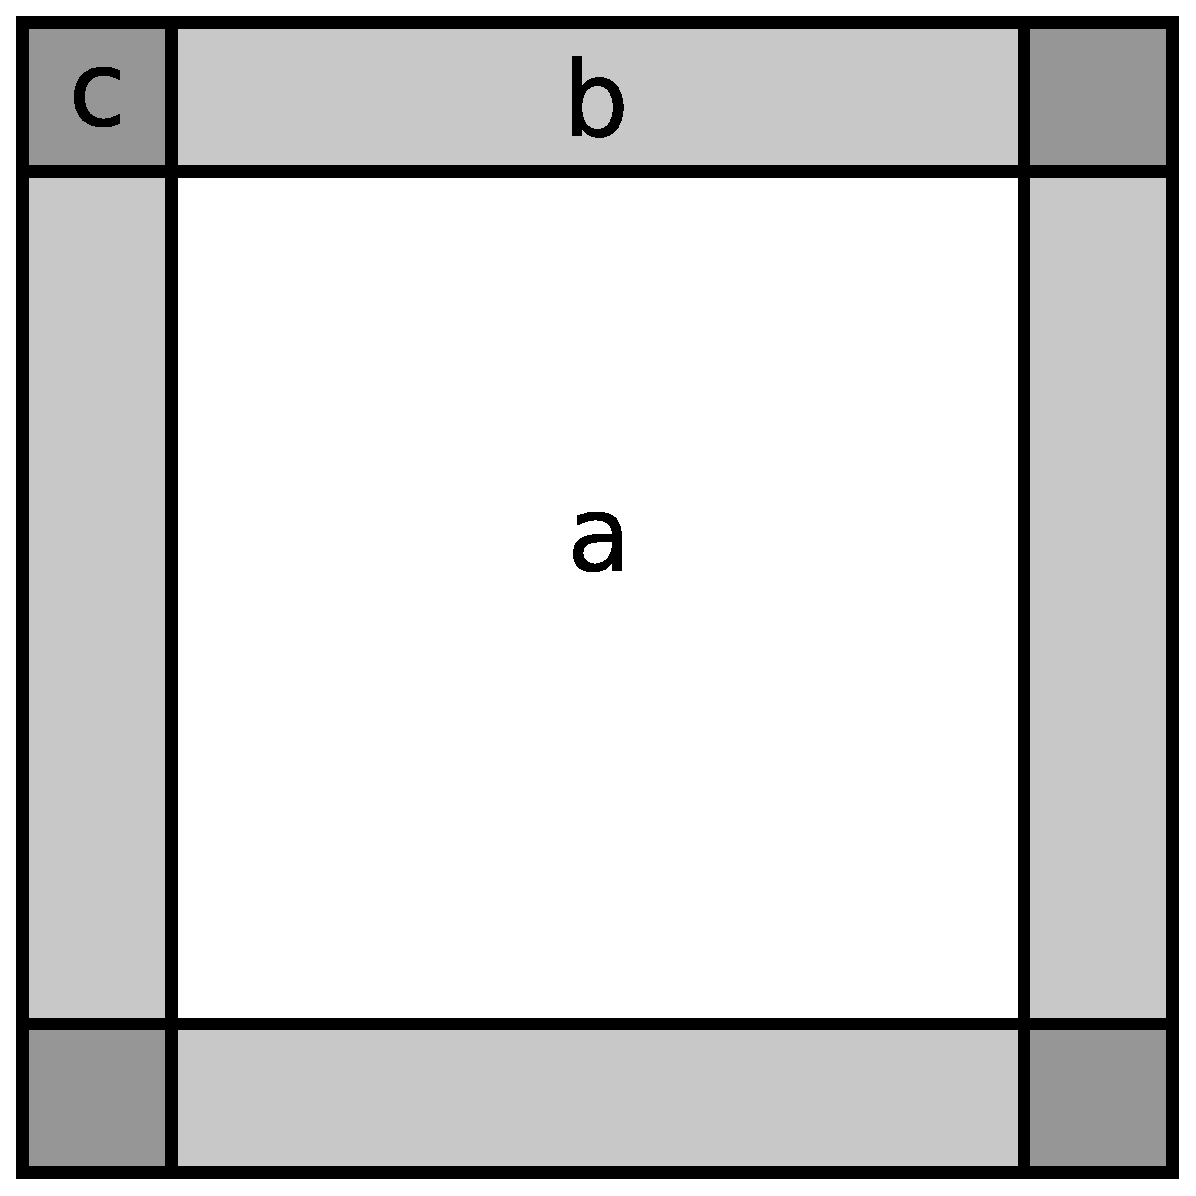
\includegraphics[width=0.5\linewidth]{PML.eps}
\caption{Placement of the PML in a two-dimensional domain. In (a), no PML is present and thus no material constants have been chosen or modified. The area marked by (b) is where the PML for the $y$ direction has been placed, waves will be attenuated in this region to prevent them from reflecting from the boundary of the domain. The PMLs in the $x$ and $y$ directions overlap in (c).}
\label{fig:PML}
\end{figure}

To create these PMLs, we introduce fictitious dielectric constants and permeabilities---in the same form as before---for each direction, which are functions of position in any spatial direction, $r\in\{x,y,z\}$,
\begin{equation}
\label{eq:fictitious}
\begin{aligned}
\varepsilon_{Fm}^*(r) &= \varepsilon_{Fm}(r)+\frac{\sigma_{Dm}(r)}{i\omega\varepsilon_0},\\
\mu_{Fm}^*(r) &= \mu_{Fm}(r)+\frac{\sigma_{Hm}(r)}{i\omega\mu_0},\\
\mathrm{for}&~m\in\{x,y,z\},
\end{aligned}
\end{equation}
where $\sigma_{Dm}$ denotes the electric conductivity in the $m$ direction, and $\sigma_{Hm}$ denotes the magnetic conductivity in the $m$ direction. Note that $m$ and $r$ are independent. The spatial dependence is denoted by $r$, which can be any of the three spatial coordinates $\{x,y,z\}$. However, $m$ denotes the direction that the constant applies in. For example, $\varepsilon_{Fx}^*(y)$ denotes the $x$-axis dielectric constant as a function of $y$, which may change with $y$, but not with $x$ or $z$. It is very important to note that $\varepsilon_{Fm}^*$ and $\mu_{Fm}^*$ have nothing at all to do with $\varepsilon_r^*$, introduced in Eq.~\ref{eq:epsilon_form}, the relative permittivity of the propagation medium. These fictitious constants only apply in the PMLs, which reside near the boundaries of the computational domain.

We introduce $\bm{\varepsilon_F^*}(\mathbf{r})$ and $\bm{\mu_F^*}(\mathbf{r})$, which are functions of position,
\renewcommand{\arraystretch}{1.75}
\begin{subequations}
\begin{equation}
\bm{\varepsilon_F^*}=\begin{bmatrix}
\varepsilon_{Fx}^*(x)\cdot\varepsilon_{Fx}^*(y)\cdot\varepsilon_{Fx}^*(z)\\
\varepsilon_{Fy}^*(x)\cdot\varepsilon_{Fy}^*(y)\cdot\varepsilon_{Fy}^*(z)\\
\varepsilon_{Fz}^*(x)\cdot\varepsilon_{Fz}^*(y)\cdot\varepsilon_{Fz}^*(z)
\end{bmatrix},
\end{equation}
\begin{equation}
\bm{\mu_F^*}=\begin{bmatrix}
\mu_{Fx}^*(x)\cdot\mu_{Fx}^*(y)\cdot\mu_{Fx}^*(z)\\
\mu_{Fy}^*(x)\cdot\mu_{Fy}^*(y)\cdot\mu_{Fy}^*(z)\\
\mu_{Fz}^*(x)\cdot\mu_{Fz}^*(y)\cdot\mu_{Fz}^*(z)
\end{bmatrix}.
\end{equation}
\end{subequations}
Which, after transforming Eqs.~\ref{eq:dH_dt},~\ref{eq:D_time},~and~\ref{eq:dD_dt} to the frequency domain---which requires identities derived in Appendices~\ref{ap:fourier1}~and~\ref{ap:fourier2}---allows us to write
\begin{subequations}
\begin{empheq}[box=\fbox]{align}
\label{eq:PML_H_w}i\omega\bm{\mu_F^*}\odot&\mathbf{H}(\omega) = -c_0\curl{\mathbf{\tilde{E}}(\omega)},\\
\label{eq:PML_D_w_H}i\omega\bm{\varepsilon_F^*}\odot&\mathbf{\tilde{D}}(\omega) = c_0\curl{\mathbf{H}(\omega)},\\
\label{eq:PML_D_w_E}\mathbf{\tilde{D}}(\omega) &= \varepsilon_r(\omega)\mathbf{\tilde{E}}(\omega) + \frac{\sigma}{i\omega\varepsilon_0}\mathbf{\tilde{E}}(\omega).
\end{empheq}
\end{subequations}
Where $\odot$ denotes the Hadamard product (elementwise product). This is the restatement of Maxwell's equations in the frequency domain in the context of a PML\@. We must be state them in the frequency domain first, since our assumed form of $\varepsilon_{Fm}^*$ and $\mu_{Fm}^*$ are frequency-dependent, shown in Eq.~\ref{eq:fictitious}. As before, only Eq.~\ref{eq:PML_D_w_E} contains information about the propagation medium. However, this time Eqs.~\ref{eq:PML_H_w}~and~\ref{eq:PML_D_w_H} are the only equations to contain information about the PML\@.

There are two restrictions for these fictitious constants to form a PML~\cite{Sacks95},
\begin{enumerate}
\item The impedance must be constant across the boundary of the PML,
\begin{equation}
\eta_0=\eta_m=\sqrt{\frac{\mu_{Fm}^*(r)}{\varepsilon_{Fm}^*(r)}},
\end{equation}
where $\eta_0$ is the impedance of the non-PML domain, shown as (a) in Fig.~\ref{fig:PML}. Since we are working in Gaussian units~\cite{Sullivan00,Kitano06},
\begin{equation}
\eta_0=1.
\end{equation}
\item The constants for the directions perpendicular to the boundary must be the inverse of the constants in the transverse directions,
\begin{equation}
\begin{aligned}
\label{eq:condition2}
\varepsilon_{Fm_\perp}^*(r)&=\frac{1}{\varepsilon_{Fm_\parallel}^*(r)}~\forall m_\parallel,\\
\mu_{Fm_\perp}^*(r)&=\frac{1}{\mu_{Fm_\parallel}^*(r)}~\forall m_\parallel.
\end{aligned}
\end{equation}
Where $m_\perp$ denotes the direction of perpendicular to the boundary and $m_\parallel$ denotes all of the directions parallel to the boundary. For example, in region (b) in Fig.~\ref{fig:PML}, the direction perpendicular to the boundary is $m_\perp=y$, and the transverse direction in the two-dimensional case would be $m_\parallel=x$ (in the three-dimensional case we would also need to include the $m_\parallel=z$ direction). So for this example, $\varepsilon_{Fy}^*(r)=1/\varepsilon_{Fx}^*(r)$ and $\mu_{Fy}^*(r)=1/\mu_{Fx}^*(r)$.
\end{enumerate}
To satisfy both of these conditions, we may choose, for all of the parallel coordinates,
\begin{equation}
\begin{aligned}
\varepsilon_{Fm_\parallel}(r)&=\mu_{Fm_\parallel}(r)=1,\\
\sigma_{Dm_\parallel}(r) &= \sigma_{D}(r),\\
\sigma_{Hm_\parallel}(r) &= \frac{\mu_0}{\varepsilon_0}\sigma_{D}(r).
\end{aligned}
\end{equation}
Substituting this into Eq.~\ref{eq:fictitious} and using Eq.~\ref{eq:condition2} to find the constants in the perpendicular direction yields
\begin{subequations}
\begin{align}
&\left\{
\begin{aligned}
\varepsilon_{Fm_\parallel}^*(r)&=1+\frac{\sigma_{D}(r)}{i\omega\varepsilon_0}\\
\mu_{Fm_\parallel}^*(r)&=1+\frac{\sigma_{D}(r)}{i\omega\varepsilon_0}
\end{aligned}\right.,\\
&\left\{
\begin{aligned}
\varepsilon_{Fm_\perp}^*(r)&=\left(1+\frac{\sigma_{D}(r)}{i\omega\varepsilon_0}\right)^{-1}\\
\mu_{Fm_\perp}^*(r)&=\left(1+\frac{\sigma_{D}(r)}{i\omega\varepsilon_0}\right)^{-1}
\end{aligned}\right..
\end{align}
\end{subequations}
Which clearly satisfies both conditions.

By gradually increasing $\sigma_{D}$ in the PML, waves in the PML will be attenuated due to Eqs.~\ref{eq:PML_H_w}~and~\ref{eq:PML_D_w_H}. We have not transformed Eqs.~\ref{eq:PML_H_w},~\ref{eq:PML_D_w_H},~and~\ref{eq:PML_D_w_E} back into the time domain, since doing so is tricky and can be done after the dimensionality for an implementation is chosen.

\section{Heterogeneous Media}
While it has not been explicitly stated, all of the material constants pertaining to the propgation medium may be spatially dependent. We have already seen that the fictitious material constants of the PML were spatially dependent in order to attenuate waves. In Eq.~\ref{eq:D_time}~and~\ref{eq:PML_D_w_E}, $\varepsilon_r$ and $\sigma$ may be written as functions of position, $\mathbf{r}$. Consequently, in the formulation of FDTD in one-dimension, $\varepsilon_r$ and $\sigma$ could have been written as $\varepsilon_r(z_i)$ and $\sigma(z_i)$ respectively.

\section{Formulation of FDTD in Two Dimensions with PML}
Before we transform Eqs.~\ref{eq:PML_H_w},~\ref{eq:PML_D_w_H},~and~\ref{eq:PML_D_w_E} back into the time domain and discretize them, we must choose between the transverse magnetic (TM) mode and transverse electric (TE) mode. For waves propagating in the $xy$-plane, the fields involved with each mode are
\begin{subequations}
\begin{equation}
\mathrm{TM}~\left\{\begin{split}
\tilde{E_z}\\
H_x\\
H_y
\end{split}\right.,
\end{equation}
\begin{equation}
\mathrm{TE}~\left\{\begin{split}
H_z\\
\tilde{E_x}\\
\tilde{E_y}
\end{split}\right..
\end{equation}
\end{subequations}
Arbitrarily, again, we will choose the TM mode. We start by implementing the PML in the $x$ direction,
\begin{subequations}
\begin{equation}
\textit{PML}_x~\left\{\begin{split}
\varepsilon_{Fx}^*(x)=\mu_{Fx}^*(x)&=\left(1+\frac{\sigma_D(x)}{i\omega\varepsilon_0}\right)^{-1}\\
\varepsilon_{Fy}^*(x)=\mu_{Fy}^*(x)&=1+\frac{\sigma_D(x)}{i\omega\varepsilon_0}\\
\varepsilon_{Fz}^*(x)=\mu_{Fz}^*(x)&=1+\frac{\sigma_D(x)}{i\omega\varepsilon_0}
\end{split}\right..
\end{equation}
\end{subequations}
And similarly for the $y$ direction,
\begin{subequations}
\begin{equation}
\textit{PML}_y~\left\{\begin{split}
\varepsilon_{Fy}^*(y)=\mu_{Fy}^*(y)&=\left(1+\frac{\sigma_D(y)}{i\omega\varepsilon_0}\right)^{-1}\\
\varepsilon_{Fx}^*(y)=\mu_{Fx}^*(y)&=1+\frac{\sigma_D(y)}{i\omega\varepsilon_0}\\
\varepsilon_{Fz}^*(y)=\mu_{Fz}^*(y)&=1+\frac{\sigma_D(y)}{i\omega\varepsilon_0}
\end{split}\right..
\end{equation}
\end{subequations}
Since the waves will propagate in the $xy$-plane, there is no $z$ dependence in our two-dimensional formulation, so the PML is the $z$ direction is ignored,
\begin{subequations}
\begin{equation}
\textit{PML}_z~\left\{\begin{split}
\varepsilon_{Fz}^*(z)=\mu_{Fz}^*(z)&=1\\
\varepsilon_{Fx}^*(z)=\mu_{Fx}^*(z)&=1\\
\varepsilon_{Fy}^*(z)=\mu_{Fy}^*(z)&=1
\end{split}\right..
\end{equation}
\end{subequations}
 Thus, Eqs.~\ref{eq:PML_H_w},~\ref{eq:PML_D_w_H},~and~\ref{eq:PML_D_w_E} become
\begin{strip}
\begin{subequations}
\begin{align}
\label{eq:2D_TM_Hx_w}i\omega\left(1+\frac{\sigma_D(x)}{i\omega\varepsilon_0}\right)^{-1}\left(1+\frac{\sigma_D(y)}{i\omega\varepsilon_0}\right)H_x(\omega) &= -c_0\frac{\partial \tilde{E_z}}{\partial y}(\omega),\\
\label{eq:2D_TM_Hy_w}i\omega\left(1+\frac{\sigma_D(x)}{i\omega\varepsilon_0}\right)\left(1+\frac{\sigma_D(y)}{i\omega\varepsilon_0}\right)^{-1}H_y(\omega) &= c_0\frac{\partial \tilde{E_z}}{\partial x}(\omega),\\
\label{eq:2D_TM_Dz_w_H}i\omega\left(1+\frac{\sigma_D(x)}{i\omega\varepsilon_0}\right)\left(1+\frac{\sigma_D(y)}{i\omega\varepsilon_0}\right)\tilde{D_z}(\omega) &= c_0\left(\frac{\partial H_y}{\partial x}(\omega)-\frac{\partial H_x}{\partial y}(\omega)\right),\\
\label{eq:2D_TM_Dz_w_E}\tilde{D_z}(\omega)&=\varepsilon_r(\omega)\tilde{E_z}(\omega)+\frac{\sigma}{i\omega\varepsilon_0}\tilde{E_z}(\omega).
\end{align}
\end{subequations}
\end{strip}

\noindent We note again the important fact that Eq.~\ref{eq:2D_TM_Dz_w_E} is the only part of this formulation to contain information about the propgation medium. All other parts, Eqs.~\ref{eq:2D_TM_Hx_w},~\ref{eq:2D_TM_Hy_w},~and~\ref{eq:2D_TM_Dz_w_H}, only contain information about propagation in free space and the PML.

Now, we transform these expressions to the time-domain, treating Eq.~\ref{eq:2D_TM_Dz_w_E} exactly as in previous discussions,
\begin{strip}
\begin{subequations}
\begin{align}
\end{align}
\end{subequations}
\end{strip}


\bibliography{References}
\bibliographystyle{ieeetr}
\newpage
\onecolumn
\appendix
\section{Inverse Fourier Transform of $E(\omega)/i\omega$}
\label{ap:fourier1}

First, we must develop some Fourier transforms of useful functions. Starting with the constant function, $x(t)=a$. Instead of directly evaluating the transform, we instead look at the inverse transform of $X(\omega)$,
\begin{equation*}
\mathcal{F}^{-1}(X(\omega))=x(t)=a=\frac{1}{2\pi}\int_{-\infty}^{\infty}X(\omega)e^{i\omega t}d\omega.
\end{equation*}
Clearly, then $X(\omega)$ must be $2\pi a\delta(\omega)$. So,
\begin{equation}
a\rightleftharpoons 2\pi a\delta(\omega).
\end{equation}
Now, we examine the signum function,
\begin{equation}
\mathit{sgn}(t) =
    \begin{cases}
    +1~&\mathrm{if}~t>0 \\
    0~&\mathrm{if}~t=0  \\
    -1~&\mathrm{if}~t<0 \\
    \end{cases}.
\end{equation}
Which has the property
\begin{equation}
\frac{d}{dt}\mathit{sgn}(t) = 2\delta(t).
\end{equation}
Taking the Fourier transform of this function follows, using integration by parts
\begin{equation*}
\begin{aligned}
\mathcal{F}(\mathit{sgn}(t))&= \int_{-\infty}^{\infty}\mathit{sgn}(t)e^{-i\omega t}dt \\
&= \left.\frac{-1}{i\omega}\mathit{sgn}(t)e^{-i\omega t}\right|_{-\infty}^{\infty} - \int_{-\infty}^{\infty}\frac{-2}{i\omega}\delta(t)e^{-i\omega t}dt \\
&= \frac{2}{i\omega}.
\end{aligned}
\end{equation*}
So,
\begin{equation}
\mathit{sgn}(t)\rightleftharpoons\frac{2}{i\omega}.
\end{equation}
The last function we need is the Heaviside step function,
\begin{equation}
H(t) =
    \begin{cases}
    1~&\mathrm{if}~t\geq0 \\
    0~&\mathrm{if}~t<0
    \end{cases}.
\end{equation}
Noticing that $H(t)=\frac{\mathit{sgn}(t)+1}{2}$ we take the Fourier transform of $H$,
\begin{equation*}
\begin{aligned}
\mathcal{F}(H(t))&=\mathcal{F}\left(\frac{\mathit{sgn}(t)+1}{2}\right) \\
&=\mathcal{F}\left(\frac{\mathit{sgn}(t)}{2}\right)+\mathcal{F}\left(\frac{1}{2}\right) \\
&= \frac{1}{i\omega}+\pi\delta(\omega).
\end{aligned}
\end{equation*}
So,
\begin{equation}
H(t)\rightleftharpoons\frac{1}{i\omega}+\pi\delta(\omega).
\end{equation}

Now, consider a general function, $f(t)$ which can be written as the integral from $-\infty$ to $t$ of some other function, $g(t)$,
\begin{equation}
f(t)=\int_{-\infty}^{t}g(\tau)d\tau.
\end{equation}
This can be expressed as a convolution integral with the Heaviside function,
\begin{equation}
f(t)=\int_{-\infty}^{t}g(\tau)d\tau = \int_{-\infty}^{\infty}g(\tau)H(t-\tau)d\tau=(g*H)(t).
\end{equation}
Fourier's convolution theorem states that for any two functions, $\theta(t)$ and $\varphi(t)$, whose Fourier transforms exist,
\begin{equation}
\mathcal{F}((\theta*\varphi)(t)) = \Theta(\omega)\varPhi(\omega).
\end{equation}
Applying this to our function, $f(t)$, yields,
\begin{equation}
\mathcal{F}(f(t)) = G(\omega)\left[\frac{1}{i\omega}+\pi\delta(\omega)\right].
\end{equation}
So,
\begin{equation}
\int_{-\infty}^{t}g(\tau)d\tau\rightleftharpoons G(\omega)\left[\frac{1}{i\omega}+\pi\delta(\omega)\right].
\end{equation}
Finally, we can use this identity to find $\mathbf{E}(t)$, given $\mathbf{E}(\omega)$. We apply the above identity to each of the components of $\mathbf{E(\omega)}\left[\frac{1}{i\omega}+\pi\delta(\omega)\right]$. Then,
\begin{equation}
\int_{-\infty}^{t}\mathbf{E}(\tau)d\tau\rightleftharpoons \mathbf{E}(\omega)\left[\frac{1}{i\omega}+\pi\delta(\omega)\right].
\end{equation}
We may assume that $\mathbf{E}(t)$ is zero for $t<0$ and $\lim_{\omega\rightarrow 0}\mathbf{E}(\omega)=0$, in which case the above equation reduces to the desired identity,
\begin{equation}
\int_0^t\mathbf{E}(\tau)d\tau\rightleftharpoons \frac{\mathbf{E}(\omega)}{i\omega}.
\end{equation}
\newpage
\section{Fourier Transform of $df/dt$}
\label{ap:fourier2}
Given a function $f(t)$ and its Fourier transform $F(\omega)$ with the condition $\lim_{t\rightarrow 0}f(t) = 0$, the Fourier transform of its first derivative, $df/dt$ is found with integration by parts,
\begin{align*}
\mathcal{F}\left(\frac{df}{dt}(t)\right) &= \int_{-\infty}^{\infty}\frac{df}{dt}(t)e^{-i\omega t}dt \\
& = \left.f(t)e^{-i\omega t}\right|_{-\infty}^{\infty} + \int_{-\infty}^{\infty}f(t)i\omega e^{-i\omega t}dt\\
& = i\omega \int_{-\infty}^{\infty}f(t)e^{-i\omega t}dt\\
& = i\omega F(\omega).
\end{align*}
Which is the identity,
\begin{equation}
\frac{df}{dt}(t) \rightleftharpoons i\omega F(\omega).
\end{equation}

\newpage
\section{The Lagrange Remainder Theorem}
\label{ap:lagrange}
\begin{theorem}
\label{thm:lagrange}
Let $f(x)$ be a function which is continuous on $[a,b]$ and $(n+1)$ differientiable on $(a,b)$. Then, for each $x\in[a,b]$ there exists $\eta\in[a,b]$ such that\footnote{The final term in this equation is called the Lagrange remainder of the $n^\mathrm{th}$ Taylor polynomial of $f$. This is because it is the error between $f$ and the $n^\mathrm{th}$ Taylor polynomial of $f$, $T_n$. That is to say, \\$f(x)-T_n(x) = \frac{f^{(n+1)}(\eta)}{(n+1)!}~\mathrm{for~some}~\eta\in[a,b]$}
\begin{equation}
f(x) = f(a) + f'(a)(x-a) + \frac{f''(a)}{2}(x-a)^2 + \cdots + \frac{f^{(n)}(a)}{n!}(x-a)^n + \frac{f^{(n+1)}(\eta)}{(n+1)!}(x-a)^{n+1}.
\label{eq:lagrange}
\end{equation}
\end{theorem}
\begin{proof}
Let $T_n$ be the $n^\mathrm{th}$ Taylor polynomial of $f$, centered at $a$. That is,
\begin{equation}
T_n(x) = f(a) + f'(a)(x-a) + \frac{f''(a)}{2}(x-a)^2 + \cdots + \frac{f^{(n)}(a)}{n!}(x-a)^n.
\end{equation}
Now choose $K\in\mathbb{R}$ such that
\begin{equation}
\label{eq:K}
f(b) = T_n(b) + K(b-a)^{n+1}.
\end{equation}
We will show that this $K$ is coefficient of the final term in Eq.~\ref{eq:lagrange}. First we consider the function $F$, defined as
\begin{equation}
F(x) = f(x) - T_n(x) - K(x-a)^{n+1}.
\end{equation}
Notice that $F^{(k)}(a)=0~\mathrm{for}~k\leq n$ since
\begin{equation}
T_n^{(k)}(x) = f^{(k)}(a) + f^{(k+1)}(a)(x-a) + \cdots + \frac{f^{(n)}(a)}{(n-k)!}(x-a)^{n-k}~\mathrm{for}~k\leq n.
\end{equation}
So $T_n^{(k)}(a)=f^{(k)}(a)$ for $k\leq n$. And,
\begin{equation}
\frac{d^k}{dx^k}K(x-a)^{n+1} = \frac{K(n+1)!}{(n+1-k)!}(x-a)^{n+1-k}.
\end{equation}
This demonstrates that $F^{(k)}(a)=0~\mathrm{for}~k\leq n$. Our choice of $K$ guarantees $F(b)=0$, so we see that $F(a)=F(b)=0$. This allows us to apply Rolle's theorem to $F$. The theorem is a special case of the mean value theorem, and it states that for any function, $g$, that is continuous on $[a,b]$ and differientiable on $(a,b)$, if $g(a)=g(b)$ then there exists at least one $c\in[a,b]$ such that $g'(c)=0$. Applying this theorem to $F$ tells us that there exists a $c_1\in[a,b]$ such that $F'(c_1)=0$. Now we examine $F'$. We have shown above that $F'(a)=0$, and we have just demonstrated that $F'(c_1)=0$, thus $F'(a)=F'(c_1)=0$. Applying Rolle's theorem now to $F'$ tells us that there exists $c_2\in[a,c_1]$ such that $F''(c_2)=0$. We continue this process on the higher derivatives of $F$ up to $F^{(n+1)}$. Here, Rolle's theorem guarantees the existence of a $c_{n+1}\in[a,c_n]$ such that $F^{(n+1)}(c_{n+1})=0$. However, since $T_n^{(n+1)}\equiv 0$, we know that $F^{(n+1)}$ is
\begin{equation}
F^{(n+1)}(x) = f^{(n+1)}(x) - K(n+1)!.
\end{equation}
So, using the fact that $F^{(n+1)}(c_{n+1})=0$,
\begin{equation}
K = \frac{f^{(n+1)}(c_{n+1})}{(n+1)!}.
\end{equation}
Let $\eta=c_{n+1}$. Since $[a,c_{n+1}]\subseteq[a,c_n]\subseteq[a,c_{n-1}]\subseteq\cdots\subseteq[a,b]$, we know $\eta\in[a,b]$. Moreover, since our choice of $K$ in Eq.~\ref{eq:K} could be repeated with $b$ replaced by any $x\in[a,b]$, the entire process could be done with any point in $[a,b]$, yielding a not-necessarily different $\eta$ for each point. However, each $\eta$ would still be in $[a,b]$ since $[a,x]\subseteq[a,b]~\forall~x\in[a,b]$. Plugging this expression for $K$ back into Eq.~\ref{eq:K} shows that for each $x\in[a,b]$, there exists $\eta\in[a,b]$ such that
\begin{equation}
f(x) = f(a) + f'(a)(x-a) + \frac{f''(a)}{2}(x-a)^2 + \cdots + \frac{f^{(n)}(a)}{n!}(x-a)^n + \frac{f^{(n+1)}(\eta)}{(n+1)!}(x-a)^{n+1}.
\end{equation}
\end{proof}
\newpage
\section{Unproven Formula}
\label{ap:Sullivan}
In~\cite{Sullivan00}, the author implicitly states that the inverse Fourier transform of Eq.~\ref{eq:2D_TM_Dz_w_H} is
\begin{equation}
\label{eq:Sullivan_continuous1}
\frac{\partial \tilde{D_z}}{\partial t} + \frac{\sigma_D(x)+\sigma_D(y)}{\varepsilon_0}\tilde{D_z} + \frac{(\Delta t)^2\sigma_D(x)\sigma_D(y)}{4\varepsilon_0^2}\frac{\partial \tilde{D_z}}{\partial t} = c_0\left(\frac{\partial H_y}{\partial x}-\frac{\partial H_x}{\partial y}\right).
\end{equation}
Which suggests the identity,
\begin{equation*}
\frac{1}{i\omega}\tilde{D_z} \rightleftharpoons \frac{(\Delta t)^2}{4} \frac{\partial \tilde{D_z}}{\partial t}.
\end{equation*}
Not only is this certainly wrong, it fails to even make sense, since $\Delta t$ should only appear after discretization.

I provide my work below which lead me to this incorrect identity from the author's equations here. The author starts with (Eq. (3.23a) in \cite{Sullivan00})
\begin{equation}
\label{eq:2D_TM_Dz_w_H_app}i\omega\left(1+\frac{\sigma_D(x)}{i\omega\varepsilon_0}\right)\left(1+\frac{\sigma_D(y)}{i\omega\varepsilon_0}\right)\tilde{D_z}(\omega) &= c_0\left(\frac{\partial H_y}{\partial x}(\omega)-\frac{\partial H_x}{\partial y}(\omega)\right),
\end{equation}
which is the same as Eq.~\ref{eq:2D_TM_Dz_w_H} used in this work. Using the following definitions (Eq. 3.15  in \cite{Sullivan00})
\begin{subequations}
\begin{align}
\label{eq:g2}gi2(i) = \frac{1}{1+\sigma_D(i)\frac{\Delta t}{2\varepsilon_0}},\\
\label{eq:g3}gi3(i) = \frac{1-\sigma_D(i)\frac{\Delta t}{2\varepsilon_0}}{1+\sigma_D(i)\frac{\Delta t}{2\varepsilon_0}},
\end{align}
\end{subequations}
where $i$ is the discretized spatial coordinate, $x_i = i\Delta x$ and $y_j = j\Delta y$, the author claims that the discrete form of Eq.~\ref{eq:2D_TM_Dz_w_H_app} in the time-domain is (rewritten in the notation used in this work)
\begin{equation}
\label{eq:Sullivan_Dz}
\begin{split}
\tilde{D_z}(x_i,y_j,t_k) &= gi3(x_i)gj3(y_j)\tilde{D_z}(x_i,y_j,t_{k-1})\\
 &+ \frac{gi2(x_i)gj2(y_j)}{2}\left[H_y(x_i,y_j,t_k)-H(x_{i-1},y_j,t_k)\right.\\
&\left.-H_x(x_i,y_j,t_k)+H_x(x_i,y_{j-1},t_k)\right].
\end{split}
\end{equation}
We will work backwards to un-discretize this equation to see if this is indeed the inverse Fourier transform of Eq.~\ref{eq:2D_TM_Dz_w_H_app}. Substituting Eqs.~\ref{eq:deltat},~\ref{eq:g2},~and~\ref{eq:g3} and assuming $\Delta x = \Delta y$ yields,
\begin{equation}
\begin{split}
\tilde{D_z}(x_i,y_j,t_k) &= \left(\frac{1-\sigma_D(x_i)\frac{\Delta t}{2\varepsilon_0}}{1+\sigma_D(x_i)\frac{\Delta t}{2\varepsilon_0}}\right)\left(\frac{1-\sigma_D(y_j)\frac{\Delta t}{2\varepsilon_0}}{1+\sigma_D(y_j)\frac{\Delta t}{2\varepsilon_0}}\right)\tilde{D_z}(x_i,y_j,t_{k-1})\\
 &+ \left(1+\sigma_D(x_i)\frac{\Delta t}{2\varepsilon_0}\right)^{-1}\left(1+\sigma_D(y_j)\frac{\Delta t}{2\varepsilon_0}\right)^{-1}\frac{\Delta t}{\Delta x}c_0\left[H_y(x_i,y_j,t_k)\right. \\
&\left.-H(x_{i-1},y_j,t_k)-H_x(x_i,y_j,t_k)+H_x(x_i,y_{j-1},t_k)\right].
\end{split}
\end{equation}
The final bracketed term, over $\Delta x$, is clearly just the finite differences of $\partial H_y/\partial x$ and $\partial H_x/\partial y$ (with the assumption that $\Delta x = \Delta y$). Knowing this, multiplying both sides by $\frac{1}{\Delta t}\left(1+\sigma_D(x_i)\frac{\Delta t}{2\varepsilon_0}\right)\left(1+\sigma_D(y_j)\frac{\Delta t}{2\varepsilon_0}\right)$, and subtracting the $\tilde{D_z}(x_i,y_j,t_{k-1})$ term to the left side gives
\begin{equation}
\label{eq:substituted}
\begin{split}
&\frac{1}{\Delta t}\left[\left(1+\sigma_D(x_i)\frac{\Delta t}{2\varepsilon_0}\right)\left(1+\sigma_D(y_j)\frac{\Delta t}{2\varepsilon_0}\right)\tilde{D_z}(x_i,y_j,t_k)\right. \\
&\left.- \left(1-\sigma_D(x_i)\frac{\Delta t}{2\varepsilon_0}\right)\left(1-\sigma_D(y_j)\frac{\Delta t}{2\varepsilon_0}\right)\tilde{D_z}(x_i,y_j,t_{k-1})\right]\\
& = c_0\left(\frac{\partial H_y}{\partial x}-\frac{\partial H_x}{\partial y}\right).
\end{split}
\end{equation}
And so the right side of Eq.~\ref{eq:2D_TM_Dz_w_H_app} is recovered (since $\frac{\partial H_y}{\partial x}(\omega) \rightleftharpoons \frac{\partial H_y}{\partial x}(t)$ and likewise for $H_x$). So we work only with the left side of Eq.~\ref{eq:substituted} now, which we expect to be the inverse Fourier transform of the left side of Eq.~\ref{eq:2D_TM_Dz_w_H_app}. Fully expanding the left side shows
\begin{align*}
&\begin{aligned}
\rightarrow\frac{1}{\Delta t}&\left[\left(1+\frac{\Delta t}{2\varepsilon_0}\left(\sigma_D(x_i)+\sigma_D(y_j)\right)+\frac{\left(\Delta t\right)^2}{4\varepsilon_0^2}\sigma_D(x_i)\sigma_D(y_j)\right)\tilde{D_z}(x_i,y_j,t_k)\right.\\
&\left.-\left(1-\frac{\Delta t}{2\varepsilon_0}\left(\sigma_D(x_i)+\sigma_D(y_j)\right)+\frac{\left(\Delta t\right)^2}{4\varepsilon_0^2}\sigma_D(x_i)\sigma_D(y_j)\right)\tilde{D_z}(x_i,y_j,t_{k-1})\right],
\end{aligned}\\
&\begin{aligned}
\rightarrow \frac{\tilde{D_z}(x_i,y_j,t_k)-\tilde{D_z}(x_i,y_j,t_{k-1})}{\Delta t} &+ \frac{\sigma_D(x_i)+\sigma_D(y_j)}{\varepsilon_0}\frac{\tilde{D_z}(x_i,y_j,t_k)+\tilde{D_z}(x_i,y_j,t_{k-1})}{2}\\
& + \frac{\Delta t \sigma_D(x_i)\sigma_D(y_j)}{4\varepsilon_0^2}\left(\tilde{D_z}(x_i,y_j,t_k)-\tilde{D_z}(x_i,y_j,t_{k-1})\right).
\end{aligned}
\end{align*}
We will use the same fact the author uses,
\begin{equation}
\frac{\tilde{D_z}(x_i,y_j,t_k)+\tilde{D_z}(x_i,y_j,t_{k-1})}{2} = \tilde{D_z}(x_i,y_j,t_{k-1/2}) = \tilde{D_z}(t),
\end{equation}
meaning that $\tilde{D_z}(t)$ should be the average of the timesteps immediately before and after it. We will also use the definition of the central difference approximation, just as before, to arrive at an expression for this left side in continuous form
\begin{equation}
\label{eq:Sullivan_continuous2}
\rightarrow \frac{\partial\tilde{D_z}}{\partial t} + \frac{\sigma_D(x)+\sigma_D(y)}{\varepsilon_0}\tilde{D_z}(t) +\frac{\sigma_D(x)\sigma_D(y)\left(\Delta t\right)^2}{4\varepsilon_0^2}\frac{\partial \tilde{D_z}}{\partial t}.
\end{equation}
Which is the left side of Eq.~\ref{eq:Sullivan_continuous1} as claimed. Already this must be incorrect, since we have a $\Delta t$ in a function which is supposed to be continuous. However, now we take the Fourier transform of this and compare it to the left side of Eq.~\ref{eq:2D_TM_Dz_w_H_app}. Using the identity proven in Appendix~\ref{ap:fourier2}, we see that the Fourier transform of Eq.~\ref{eq:Sullivan_continuous2} is
\begin{equation}
\label{eq:Sullivan_continuous_w1}
i\omega\tilde{D_z}(\omega)+\frac{\sigma_D(x)+\sigma_D(y)}{\varepsilon_0}\tilde{D_z}(\omega) + \frac{\sigma_D(x)\sigma_D(y)\left(\Delta t\right)^2}{4\varepsilon_0^2}i\omega\tilde{D_z}(t).
\end{equation}
To compare it to the left side of Eq.~\ref{eq:2D_TM_Dz_w_H_app}, we expand Eq.~\ref{eq:2D_TM_Dz_w_H_app},
\begin{equation}
\label{eq:Sullivan_continuous_w2}
\rightarrow i\omega\tilde{D_z}(\omega)+\frac{\sigma_D(x)+\sigma_D(y)}{\varepsilon_0}\tilde{D_z}(\omega)+\frac{\sigma_D(x)\sigma_D(y)}{i\omega\varepsilon_0^2}\tilde{D_z}(\omega).
\end{equation}
If the author's transformation is correct and the above un-discretization and Fourier transform is correct, then Eqs.~\ref{eq:Sullivan_continuous_w1}~and~\ref{eq:Sullivan_continuous_w2} should be equivalent. Which suggests,
\begin{equation}
\Delta t = \frac{2}{i\omega}.
\end{equation}
Clearly, something is wrong here. I cannot make sense of it, and not for lack of trying.
\end{document}
